\documentclass{beamer}

\usepackage[utf8]{inputenc}
\usepackage[T1]{fontenc}
\usepackage{color}
\usepackage{textcomp}
\usepackage{graphicx}

\usepackage{beamerthemesplit}
\usetheme{esc}
\author{Valentin H\"anel}
%\email{valentin.haenel@gmx.de}
\institute{Bernstein Center for Computational Neuroscience Berlin}

\title{Git}
\definecolor{gray}{rgb}{0.10,0.10,0.10}
\date{April 2, 2009}

\begin{document}
%\frame{\titlepage}

\begin{frame}
	
\includegraphics[scale=0.05]{BCCN_logo_berlin.jpg}
	\titlepage
\end{frame}

\input{slides-01.tex}

\frame{
\frametitle{Zussamenhang}

\begin{figure}[ht]
	  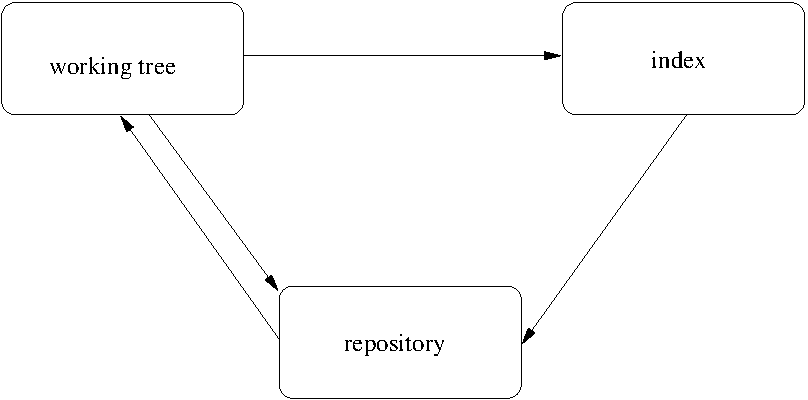
\includegraphics[scale=0.7]{git-im0.pdf}
      \caption{Zussamenhang von \textit{working tree}, \textit{index} und
      \textit{repository}}
\end{figure}
}

\input{slides-02.tex}

\frame{
\frametitle{Objects}

Ein Git \emph{repository} enthält \emph{commits} die durch ihre \emph{SHA-1 IDs} benannt
werden, \emph{commits} wiederum bestehen aus \emph{trees} und \emph{blobs}.

\begin{figure}[ht]
	  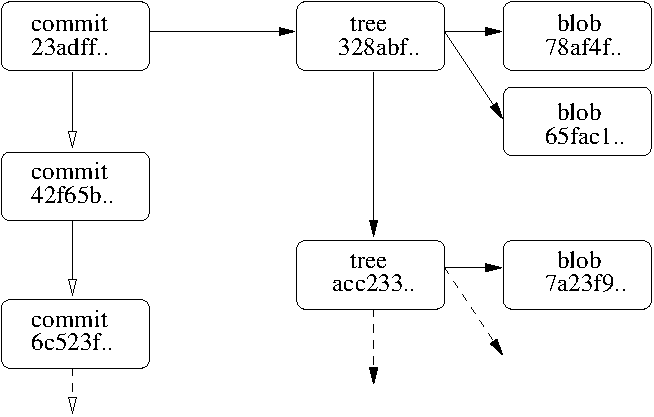
\includegraphics[scale=0.7]{git-overview.pdf}
      \caption{\emph{commits}, \emph{trees} und \emph{blobs}}
\end{figure}
}



\input{slides-03.tex}

\frame{
\frametitle{Transport Kommandos}

\begin{figure}[ht]
	  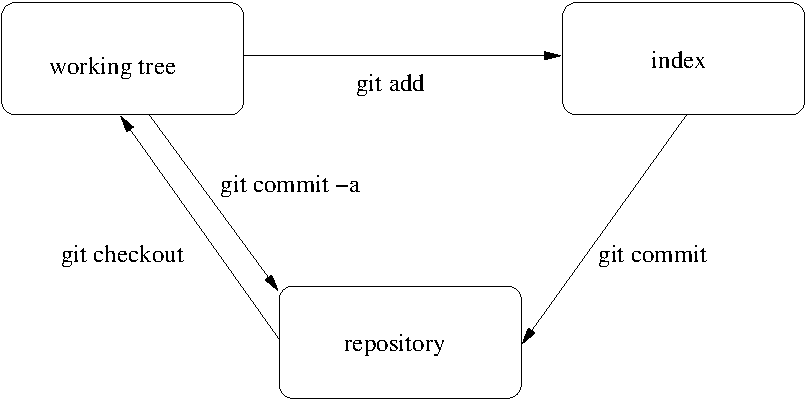
\includegraphics[scale=0.7]{git-im1.pdf}
      \caption{Zusammenhang von {\tt git-add}, {\tt git-commit} und {\tt git checkout}}
\end{figure}
}

\section{Suchen und Finden}

%\input{slides-04.tex}A

\frame{
\frametitle{\textit{commits} sind das Geheimniss}

\begin{itemize}
    \item Wie ihr vielleicht schon erahnen, könnt sind \textit{commits} das
        Geheimniss um Git wirklich zu verstehen.
    \item Viele Git Kommandos akzeptieren einen \textit{commit}, und es gibt ein
        paar Alternativen (zu der lästigen 40-Zeichen-Sequenz) um diese zu benennen
    \item Meistens reicht f\"ur die Angabe von einem \textit{commit} die ersten 4-7
        Zeichen des \textit{object name}
    \item @HEAD@ ist eine implzite Referenz zu dem aktuellsten \textit{commit}
    \item Relative Angaben werden mit \^{} und $\sim$ gemacht
    \item z.B. {\tt HEAD\^{}\^{}\^{}} und {\tt HEAD$\sim$3} sind equivalent und
        beschreiben beide den dritten \textit{commit} vor {\tt HEAD}
\end{itemize}
}

\section{Suchen}

\begin{frame}[fragile]
\frametitle{Einsehen des Inhaltes}

\begin{itemize}
    \item Mit \emph{git log} kann man sich alle bisherigen \textit{commits} anzeigen lassen
    \item Es gibt eine Vielzahl von Möglichkeiten die Ausgabe zu verändern:

\hspace{0.5cm}

    \item
\begin{tabular}{ l l }
{\tt git log -N}                            & die letzten @N@ anzeigen\\
{\tt git log COMMIT}                        & bis zu @COMMIT@ anzeigen \\
{\tt git log --since="23 hours"}            & alle seit ... \\
{\tt git log --before="42 days"}            & alle vor ... \\
{\tt git log --pretty=oneline}              & eine Zeile pro \textit{Zeile} \\
{\tt git log A..B}                          & alle zwischen {\tt A} und {\tt B}
\end{tabular}

\hspace{0.5cm}

\item{

\begin{verbatim}
commit b99336317088ba4ae40e45c338c6981e3f402f8e
Author: Valentin Haenel <valentin@cs.tu-berlin.de>
Date:   Sun Apr 5 20:19:50 2009 +0200

adding slides about git-log
\end{verbatim}

}

\end{itemize}

\end{frame}

\input{slides-05.tex}

\frame{
\frametitle{Branch}

\begin{itemize}
    \item \textit{branches} haben namen
    \item Der Name von einem \textit{branch} ist eine Referenz zu einem  \textit{commit}
    \item Dieser \textit{commit} hat Vorfahren
\end{itemize}


\begin{figure}[ht]
	  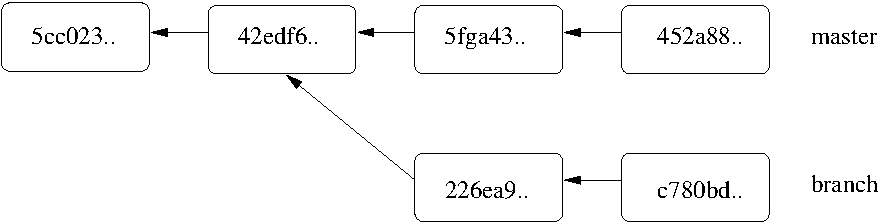
\includegraphics[scale=0.7]{git-branch.pdf}
      \caption{Graphische Darstellung von einem \textit{branch}}
\end{figure}
}

\input{slides-06.tex}


\begin{frame}[fragile]
\frametitle{Inhalt von .git}

git speichert alles in dem Verzeichniss {\tt.git/} auch bekannt als \textbf{git
directory}

\begin{verbatim}
    % tree -L 1  .git/
    .
    |-- HEAD            # der gegenwärtige HEAD
    |-- config          # Konfiguration (user, email)
    |-- index           # der index
    |-- objects         # die eigentlichen Objekte

\end{verbatim}

\end{frame}


\end{document}
